\section{Project Management}
To effectively manage time within this project of large nature and short time frame, several project management methodologies and principals were implemented. In order to select the correct approach to incorporate project management into this project, methodologies were chosen based on the projects needs. Time within the project needed to be allocated towards both theoretical and technical research, to select the technologies to be used, models for evaluation and to learn how to use the technologies to implement them. As well as this, time should also be invested into the implementation and training of the models used in this evaluation, this will ensure fair and accurate results, and ample time to perform training. The selected methodology should also allow for flexibility, if issues arise or any risks identified occur, the project can remain on track.

A kanban style approach was the selected project management methodology that met the above needs. The kanban approach is an agile methodology which divides a project into work items, which are then represented on a kanban board, splitting the work items into three categories: to do, in progress and complete. This is used along side its four agile inspired principles: visualise workflow, limit work in progress, focus on flow and continuous improvement. Using this approach means that project members are only ever focused on work in progress, meaning that items in the backlog, or to do section, can be re-prioritised and changed without impacting the project, allowing for continuous improvement of the product. Some benefits of kanban, as reported by \cite{ahmad2013kanban}, highlight a better understanding of the entire project process as the visualisation of work items give developers a clear understanding of the projects direction. Kanban's limitation of work in progress items also minimises lead time, with the likes of BBC worldwide reducing time to delivery by 37\% \citep{senapathi2011factors}.

There are some drawbacks to the kanban method however. Most drawbacks identified by \cite{ahmad2013kanban} are related to its difficulty of implementation into pre-existing work cultures and teams. Since this project has a singular developer, these are not applicable. One drawback that this project must be mindful of is introduced by the lack of timing attached to work items, meaning that if not monitored correctly, the project could fall behind schedule due to over focusing on one work item. In order to mitigate these risks, some guidelines from the waterfall methodology were implemented into the project, namely it sequential project structure principle. The reasoning behind this combined approach allows for the limited multitasking and flexibility that kanban introduces combined with the set time planning of waterfall. In the context of this project, it will allow flexibility and adaptability, if the projects priorities change following regular supervisor meetings, or if issues occur. It will also allow constant iteration and improvement of models being evaluated while not being overwhelmed by multitasking.

While abiding by the guiding principles mentioned above, the project will make use of a kanban board for all work items, alongside a waterfall style Gantt chart to pre-plan the entire projects timeline, seen in \ref{fig:gantt-chart}.

\begin{figure}[H]
    \centering
    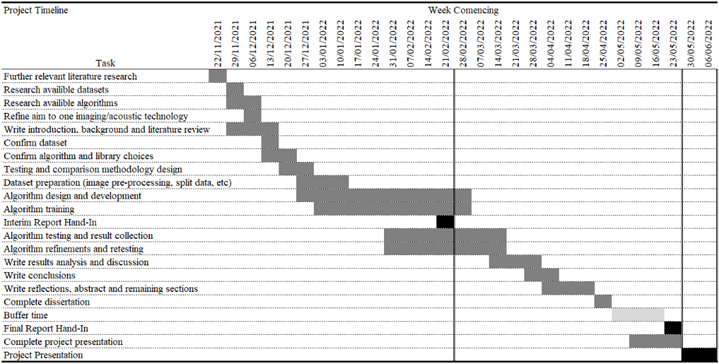
\includegraphics[width=\textwidth]{figures/gantt-chart.png}
    \caption{Project plan presented as a Gantt chart.}
    \label{fig:gantt-chart}
\end{figure}

\section{Software Development}
Text

\section{Toolsets and Machine Environments}
There are a number of toolsets used within this projects artefact, both software and hardware related. In order to reproduce the artefact, these must be installed as prerequisites to the project.

\subsection{Software Requirements}
The following sections introduce the software used to complete this research project. While some software, like the development environments and visualisation software like TensorBoard are optional and are not needed to train the models, some modification to the code might be needed to run without them.

\phantomsection

\subsubsection{Python}
Python was the chosen language for this project, due to a number for reasons. Firstly Python is the most popular programming language worldwide, with a 27.95\% market share, according to the PYPL index \citep{PYPLPopu3:online}. This means not only is it well known by computer and data scientists, it is also well supported by both its richness of available libraries and its documentation. Its popularity directly influences its choice for project, by allowing others to pick up and further improve on findings from this research. Other languages in the PYPL list, such as Java, JavaScript and C\# also have a large community and wide documentation, however there are still other factors that set Python apart from these, making it the final choice. 

Python's availability of libraries is also a direct influence of choice for this project, as the majority of machine learning and deep learning libraries are supported by Python, such as TensorFlow, PyTorch and Scikit-Learn, with its dominance expected to remain for the foreseeable future \citep{raschka2020machine}. This is compared to libraries like DeepLearning4j, a deep learning library for Java, which, while comparable to the Python libraries, has a declining use within the medical field \citep{erickson2017toolkits}. 

Finally Python has a very natural syntax which is very close to the English language, making it very readable, even by those with no prior knowledge of the language, compared to the likes of Java and C\# \citep{srinath2017python}.

The entirety of the projects code was written in Python and such is a hard requirement to run the projects artefact. It is recommended to use Python 3.7 or later for TensorFlow support.

\subsubsection{TensorFlow - Keras}
TensorFlow with Keras as the API layer was the chosen machine learning library for this project. TensorFlow is an "end-to-end open source platform for machine learning" with an eager execution environment \citep{TensorFl5:online}. TensorFlow is built upon tensors, which are immutable, multi-dimensional arrays, that are used to store objects, classes and weights that propagate through neural networks. TensorFlow was chosen over other libraries like PyTorch and SciKit-Learn for several reasons, one such reason is due to is eager execution, which means one can view results of operations instantly, as tensors are updated as they are called upon within the code. This allows one to quickly judge the success of a particular model instantly, as it trains, resulting in quick debugging. Another reason for choosing TensorFlow, was its integration with Keras, an API written to run on top of TensorFlow, which makes the creation of machine learning models simple and fast with its sequential model \citep{AboutKer65:online}. The sequential model is a linear stack of layers which allows a user to prototype and build models from scratch, or improve on an existing library of models easily. Keras supplies over 30 pre-trained deep learning models for use within its API, this is a key feature in this project as it allows for accurate replication of the chosen models for evaluation and use of transfer learning in selected models.

TensorFlow and Keras are amongst the most popular machine learning libraries for research studies and business use cases, making both its development support and its applicability in real world use cases beat out competitors. \cite{hale2018deep} ranked each library against each other based on a power score, calculated by the weighted scores of popularity from multiple data sources. 

\begin{figure}[H]
    \centering
    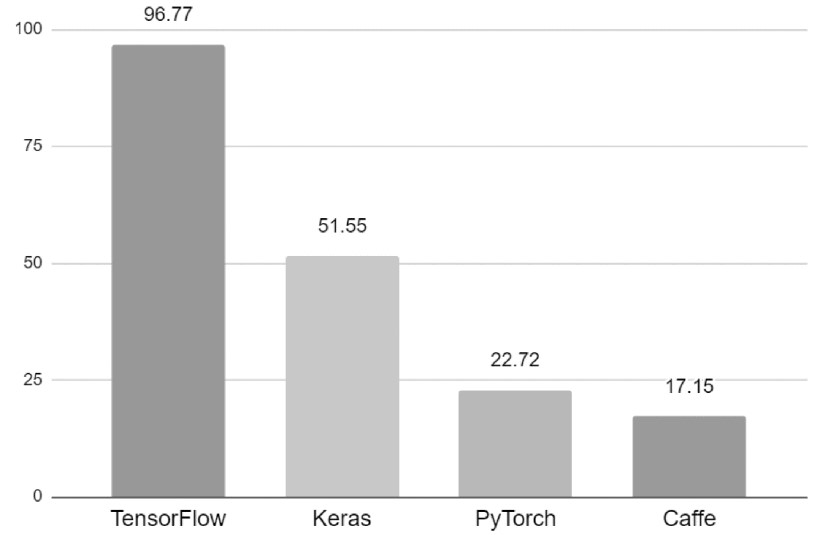
\includegraphics[width=0.65\textwidth]{figures/ml-power-sources.jpg}
    \caption{Power scores of various machine learning libraries \citep{hale2018deep}.}
    \label{fig:ml-power-scores}
\end{figure}

The TensorFlow and Keras are used in the entirety of this project and such is a hard requirement to run the artefact. It is recommended to use TensorFlow 2.0 and Keras 2.0 or later, but with some code modifications, TensorFlow 1.0+ and Keras 1.0+ can also be used.

\subsubsection{TensorBoard}
TensorBoard is a visualisation library for TensorFlow, that tracks and plots metrics from TensorFlow models as they train \citep{TensorBo28:online}. Within this project, TensorBoard was used to both extract visual data of the models performs, like accuracy and loss metrics, as well as tracking weather a particular model was over/under fitting. TensorBoard was chosen over other visualisation libraries like Matplotlib or seaborn due to it's tight integration with TensorFlow, and interactivity. TensorBoard also allows one to implement and track hyper-parameter tuning within a project, this was extremely beneficial for this project.

In this project, TensorBoard 2.8.0 was used and is a hard requirement to run the artefact. As with TensorFlow, it is recommended to use TensorBoard 2.0 or later, but with some code modifications, TensorBoard 1.0+ can also be used.

\subsubsection{Scikit-Learn}
Scikit-Learn is a machine learning library built for Python, which is bundled with many evaluation functions \citep{33Metric9:online} and cross validation functions \citep{31Crossv34:online}. The evaluation functions used within Scikit-Learn provided accuracy, precision, recall, F1 score and confusion matrix metrics, for each trained model in the project. Scikit-Learn's evaluation functions were chosen over Keras' inbuilt functions as Keras' own evaluation functions are limited to only providing loss and accuracy data\citep{Modeltra48:online}, with other metrics having to be calculated manually, making Scikit-Learn a faster and easier to implement solution. 

Scikit-Learn's Stratified K-Fold cross validation implementation was also used within this project. This is used to ensure fairness when evaluating models performance, by taking an average of each folds validation accuracy', the possibility of dataset or training inconsistencies are removed. Keras offers no in built solution to cross validation, so much like the evaluation metrics, has to be performed manually, making Scikit-Learn a faster and easier to implement solution.

Scikit-Learn was also used to shuffle and re-sample the training data, so that there was no bias towards a particular class or model due to possible bias in the dataset structure.

In this project, Scikit-Learn 1.0.2 was used and is a hard requirement to run the artefact.

\subsubsection{Pandas}
Pandas is an open source data manipulation and analysis library for Python \citep{pandasPy63:online}. Pandas was used for loading in the dataset to the artefact, performing some initial pre-processing, like dropping any patient data from the dataset, to remove bloat. Pandas was also used to store and handle the dataset throughout the artefact, using pandas DataFrames, a two dimensional data structure to store tabular data, like the datasets labels.

In this project, pandas 1.3.5 was used and is a hard requirement to run the artefact.

\subsubsection{NumPy}
NumPy is an open source scientific and mathematics library for Python \citep{NumPy90:online}. NumPy was used for basic numerical operations within the project, and is also a dependency for other libraries used. In this project, NumPy 1.21.6 was used and is a hard requirement to run the artefact.

\subsubsection{Google Cloud Platform - Development Environment}
Google Cloud Platform was used in this project to train and test the initial selection of the six COVID-19 classification models and perform hyper-parameter tuning on each model. Two services used within Google Cloud Platform were Vertex AI \citep{VertexAI57:online} and Cloud Storage \citep{CloudSto72:online}. Vertex AI enables fast code building though Vertex AI Workbench, a Jupyter notebook environment with access to server grade GPUs. This enabled quick testing and finalisation of the first round of models for evaluation within this project. Vertex AI also has the ability to execute notebook runs on specific hardware and software instances in parallel, meaning fairness though out the first stages of model evaluation and a fast time to results thanks to the allocated NVIDIA Tesla K80s for each instance. Cloud storage was used to store the COVIDx-CXR database the models were trained on, alongside the saved trained model weights and the TensorBoard logs.

Google Cloud Platform and its subsidiary solutions are not a requirement to run the artefact.

\subsubsection{Google Colab - Development Environment}
Text

\subsubsection{Jupyter Notebook - Development Environment}
Text

\subsubsection{GitHub}
Text

\subsection{Hardware Requirements}
While TensorFlow can run on a large number of devices, there are some hardware limitations, especially if a Graphical Processing Unit (GPU) is used to accelerate performance. TensorFlow requires a CPU capable of AVX instructions, which most modern Computational Processing Unit's (CPU) support \citep{InstallT17:online}. If GPU acceleration is required and the device used has an NVIDIA GPU, then it must support compute unified device architecture (CUDA), a "parallel computing platform" which can "dramatically speed up computing applications by harnessing the power of GPUs" \citep{CUDAZone2:online}. If the device has a GPU that does not support CUDA, but does support DirectX 12 (e.g. an AMD GPU manufactured in the last several years), then Microsoft's DirectML can be used enable GPU support for TensorFlow \citep{Introduc93:online}. Precautions must be taken if DirectML is used however, as it has differing version requirements of Python, TensorFlow and NumPy.

\section{Research Methods}
You should investigate the types of research methods necessary to validly answer the research questions that your project addresses. You should cite relevant sources to justify your choices.
\begin{itemize}
    \item abductive
    \item primary data
    
\end{itemize}